\chapter{HERMITE KUBIK MONOTON}
Pada bab ini dibahas tentang dasar untuk membentuk interpolasi yang monoton, terutama interpolasi Hermite kubik monoton yang akan digunakan sebagai basis dalam pembentukan interpolasi spline kubik monoton.
\section{Interpolasi Monoton}

Untuk membentuk interpolasi monoton, perlu didefinisikan terlebih dulu sifat monoton fungsi.

\begin{definisi}\label{definisiMonoton}
     Misal $f:[a,b] \to \R$, dengan $f(a) \leq f(b)$ $(f(a) \geq f(b))$. Fungsi $f$ disebut \textbf{monoton naik (monoton turun)} pada interval $[a,b]$ jika untuk setiap $x,y \in [a,b]$ dengan $x \leq y$ berlaku
    \begin{equation*}
        f(x) \leq f(y),\:(f(x) \geq f(y)).
    \end{equation*}
\end{definisi}
\begin{contoh}
    Diberikan sebuah fungsi \(f:[0,1] \to \R\) dengan $f(x)=x^3$, untuk setiap $x \in [0,1]$. Fungsi $f$ merupakan fungsi monoton naik pada interval $[0,1]$ karena $f(0) = 0 \leq 1 = f(1)$ dan untuk setiap $x,y \in [0,1]$ dengan $x \leq y$ berlaku
    \begin{equation*}
        f(x) = x^2 \leq y^2 = f(y).
    \end{equation*}
\end{contoh}

Interpolasi adalah metode numerik yang menghasilkan titik baru diantara titik yang diberikan. Sebuah metode interpolasi dikatakan \textbf{monoton} jika hasil interpolasi memenuhi Definisi \ref{definisiMonoton} pada setiap interval tertutup diantara titik yang diberikan.

Sebuah interpolasi yang monoton memiliki banyak kelebihan, salah satunya hasil interpolasi lebih akurat untuk data yang diinterpolasi bersifat monoton. Sebagai contoh misalkan kita memiliki data $(0,10)$, $(1,8.7)$, $(2,2.1)$, $(3,1.5)$, dan $(4,0.1)$. Apabila diplot datanya akan diperoleh grafiknya sebagai berikut.
\begin{figure}[H]
    \centering
    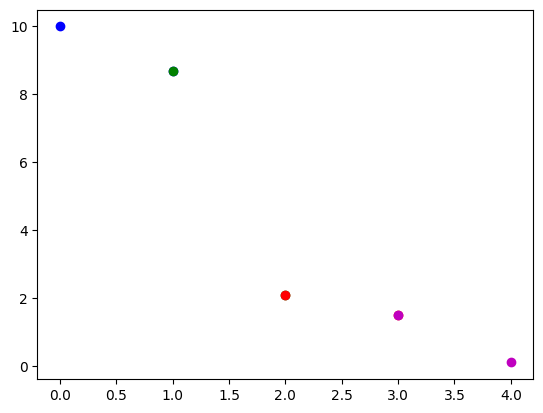
\includegraphics{Images/plotSplineKubik.png}
    \caption{Plot titik}
    \label{titik}
\end{figure}
Dari Gambar \ref{titik} dapat dilihat bahwa datanya monoton turun. Dalam menginterpolasi data tersebut, salah satu interpolasi yang dapat mempertahankan sifat monoton data adalah interpolasi linear. Dengan menggunakan metode interpolasi linear pada data, diperoleh grafik hasil interpolasinya berupa garis yang menghubungkan setiap titiknya.
\begin{figure}[H]
    \centering
    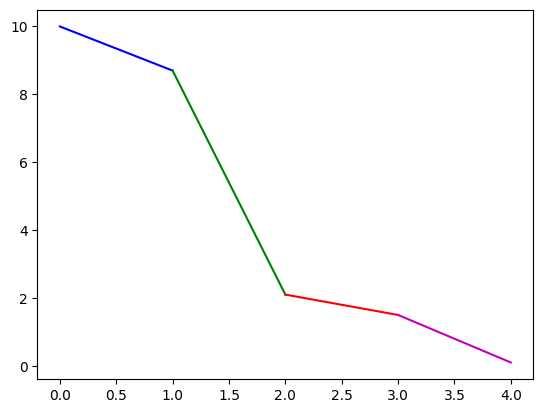
\includegraphics{Images/linear.png}
    \caption{Grafik interpolasi linear}
    \label{linear}
\end{figure}
Interpolasi linear pada Gambar \ref{linear} mempertahankan sifat monoton yang diinginkan tetapi hasil interpolasi yang diperoleh tidak dapat diturunkan pada titik-titik yang diinterpolasi.

Misalkan data yang diinterpolasikan pada Gambar \ref{titik} merupakan data kecepatan bola hingga berhenti dengan sumbu-$x$ berupa waktu dalam detik dan sumbu-$y$ berupa kecepatan bola dalam $m/s$. Jika perubahan kecepatan bola digambarkan menggunakan Gambar \ref{linear}, maka perubahan kecepatan bola pada titik data yang tidak mulus akan terjadi secara tidak wajar sehingga bola terlihat melambat secara tiba-tiba. Untuk menghindari hal tersebut data diinterpolasi menggunakan interpolasi spline kubik sehingga diperoleh grafik interpolasinya.
\begin{figure}[H]
    \centering
    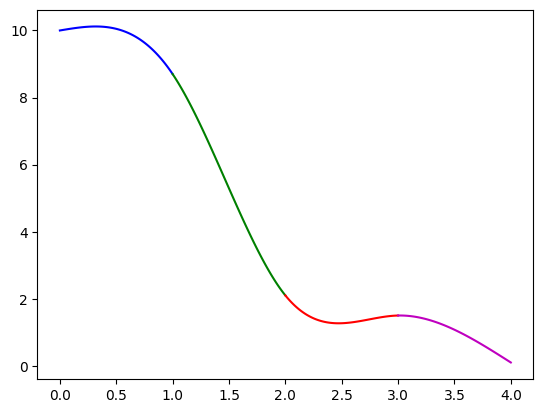
\includegraphics{Images/splineKubik.png}
    \caption{Grafik interpolasi spline kubik}
    \label{grafikHermite}
\end{figure}

Diperhatikan grafik interpolasi spline kubik pada Gambar \ref{grafikHermite} sudah terlihat mulus namun pada grafik tersebut data yang semula ingin dipertahankan sifat monotonnya menjadi hilang. Menghilangnya sifat monoton ini dapat menjadi masalah untuk nilai yang berada jauh dari nilai yang diinginkan. Seperti sebelumnya misal kita menginterpolasi data kecepatan bola tanpa menghiraukan arah bolanya, maka nilai kecepatan bola haruslah positif. Interpolasi yang tidak monoton menyebabkan nilai kecepatan bola berdasarkan hasil interpolasi dapat bernilai negatif. Hal ini menyebabkan hasil interpolasi tidak akurat.

\section{Interpolasi Hermite Kubik Monoton}
Pembentukan interpolasi spline kubik monoton diawali dengan pembentukan interpolasi Hermite kubik yang monoton. Polinomial hasil interpolasi Hermite kubik $P(x)$ pada titik-titik $x_1<\dots<x_n$ disebut monoton apabila untuk setiap $i=1,\:\dots,\:n-1$, polinomial kubik $P_i(x)$ pada interval $[x_i,x_{i+1}]$ yang didefinisikan seperti pada Persamaan \eqref{PersHermiteKubik} berupa
\begin{equation}\label{P_i}
    P_i(x)=f_i + \dot{f_i}(x-x_i) + \frac{(m_i-\dot{f_i})}{h_i}(x-x_i)^2 + \frac{(\dot{f_{i+1}}+\dot{f_i}-2m_i)}{h_i^2}(x-x_i)^2(x-x_{i+1}),
\end{equation}
merupakan polinomial yang monoton. 


Sebelum diberikan syarat interpolasi Hermite kubik dengan sifat monoton, akan diberikan terlebih dahulu syarat perlu Persamaan \eqref{P_i} hasil interpolasi Hermite kubik monoton pada interval $[x_i,x_{i+1}]$.

Berikut adalah syarat perlu agar Persamaan \eqref{P_i} monoton dengan
\begin{align*}
    sign(x) = \begin{cases}
        -1&, \quad x < 0, \\
        1&, \quad x > 0.
    \end{cases}
\end{align*}

\begin{teorema}\label{perluMonoton}
    Misal $P_i$ adalah polinomial hasil interpolasi Hermite kubik dari data $\{(x_i,f_i,\dot{f_i}),(x_{i+1},f_{i+1},\dot{f_{i+1}})\}$. Jika $P_i$ monoton pada $[x_i,x_{i+1}]$, maka 
    \begin{equation}
 sign(\dot{f_i})=sign(\dot{f_{i+1}})=sign(m_i).
    \end{equation}
    Lebih lanjut, jika $m_i=0$ maka $P_i$ konstan jika dan hanya jika $\dot{f_i}=\dot{f_{i+1}}=0$.
\end{teorema}
\begin{proof}
    Polinomial $P_i$ merupakan polinomial kubik pada interval $[x_i, x_{i+1}]$ yang monoton, sehingga diperoleh
    \begin{align*}
        \dot{f_i} = P_i'(x_i) &= \lim_{x \to x_i^+} \frac{P_i(x)-P_i(x_i)}{x-x_i}, \\
        \dot{f_{i+1}} = P_i'(x_{i+1}) &= \lim_{x \to x_{i+1}^-} \frac{P_i(x_{i+1})-P_i(x)}{x_{i+1}-x}, \\
        m_i = \frac{f(x_{i+1}) - f(x_i)}{x_{i+1}-x_i} &= \frac{P_i(x_{i+1}) - P_i(x_i)}{x_{i+1}-x_i}.
    \end{align*}
    Diperhatikan bahwa $P_i$ monoton, artinya $P_i(x) \leq P_i(y)$ atau $P_i(x) \geq P_i(y)$ untuk setiap $x,y \in [x_i,x_{i+1}]$ dengan $x \leq y$ sedemikian hingga diperoleh
    $$sign(\dot{f_i})=sign(\dot{f_{i+1}})=sign(m_i).$$

    Selanjutnya jika $m_i=0$ dan $P_i$ konstan, maka berdasarkan Persamaan \eqref{P_i} diperoleh
    \begin{align*}
        \dot{f_i} = 0, \\
        m_i-\dot{f_i} = 0, \\
        \dot{f_{i+1}}+\dot{f_i}-2m_i = 0,
    \end{align*}
    sehingga diperoleh $\dot{f_i}=\dot{f_{i+1}}=0$.

    Sebaliknya jika $m_i=\dot{f_i}=\dot{f_{i+1}}=0$ maka polinomial pada Persamaan \eqref{P_i} berbentuk
    \begin{equation*}
        P_i(x)=f_i,
    \end{equation*}
    sehingga diperoleh $P_i$ konstan.
\end{proof}

Setelah diberikan syarat perlu Persamaan \eqref{P_i} monoton pada Teorema \ref{perluMonoton}, selanjutnya akan diselidiki syarat cukup agar polinomialnya monoton. Interpolasi Hermite kubik memiliki polinomial $P_i(x)$ untuk $x \in [x_i,x_i+1]$ yang diperoleh pada Persamaan \eqref{P_i} memilki deret Taylor di titik $x=x_i$ berupa
\begin{equation}\label{taylorHermite}
\begin{split}
    P_i(x) &= P_i(x_i) + P_i'(x_i)(x-x_i) + \frac{P_i''(x_i)}{2}(x-x_i)^2 + \frac{P_i'''(x_i)}{6}(x-x_i)^3 \\
    &= f_i + \dot{f_i}(x-x_i) + \frac{(-2\dot{f_i}-\dot{f_{i+1}}+3m_i)}{h_i}(x-x_i)^2 + \frac{(\dot{f_i}+\dot{f_{i+1}}-2m_i)}{h_i^2}(x-x_i)^3,
\end{split}
\end{equation}
sehingga diperoleh
\begin{equation}\label{taylorHermite2}
    P_i'(x) = \dot{f_i} + \frac{2(-2\dot{f_i}-\dot{f_{i+1}}+3m_i)}{h_i}(x-x_i) + \frac{3(\dot{f_i}+\dot{f_{i+1}}-2m_i)}{h_i^2}(x-x_i)^2,
\end{equation}
dan
\begin{equation}
    P_i''(x) = \frac{2(-2\dot{f_i}-\dot{f_{i+1}}+3m_i)}{h_i} + \frac{6(\dot{f_i}+\dot{f_{i+1}}-2m_i)}{h_i^2}(x-x_i).
\end{equation}

Berdasarkan ketunggalan polinomial Hermite, polinomial $P_i$ yang diperoleh dari deret Taylornya adalah polinomial yang sama dengan polinomial Hermite pada Persamaan \eqref{P_i}. Untuk memudahkan penulisan selanjutnya akan definisikan \mbox{$\alpha_i := \dot{f_i}/m_i$} dan $\beta_i := \dot{f_{i+1}}/m_i$.
\begin{lemma}\label{lema1}
     Misal $P_i$ adalah polinomial hasil interpolasi Hermite kubik dari data $\{(x_i,f_i,\dot{f_i}),(x_{i+1},f_{i+1},\dot{f_{i+1}})\}$. Jika $\alpha_i + \beta_i - 2 \leq 0$, maka polinomial $P_i$ monoton pada $[x_i,x_{i+1}]$ jika dan hanya jika syarat perlu monoton pada Teorema \ref{perluMonoton} terpenuhi.
\end{lemma}

\begin{proof}    
Dengan asumsi bahwa $m_i \neq 0$ dan syarat perlu monoton pada Teorema \ref{perluMonoton} terpenuhi, ditinjau dua kasus di mana $\alpha_i + \beta_i - 2 = 0$ dan $\alpha_i + \beta_i - 2 < 0$.

Untuk kasus pertama ketika $\alpha_i + \beta_i - 2 = 0$, diperhatikan bahwa 
$$\alpha_i + \beta_i - 2 = \frac{\dot{f_{i+1}}+\dot{f_i}-2m_i}{m_i},$$ sehingga diperoleh $\dot{f_{i+1}}+\dot{f_i}-2m_i = 0$. Hal ini mengakibatkan polinomial $P_i(x)$ merupakan polinomial berderajat dua berdasarkan Persamaan \eqref{taylorHermite} dan $P_i'$ linear atau konstan. Polinomial $P_i'$ linear atau konstan sehingga pada interval $[x_{i},x_{i+1}]$ grafiknya berupa garis lurus. Hal ini berakibat pada $P_i'$ berlaku 
\begin{align*}
    \min(\dot{f_i},\dot{f_{i+1}}) \leq P_i'(x) \leq \max(\dot{f_i},\dot{f_{i+1}}),
\end{align*} 
untuk setiap $x \in [x_i,x_{i+1}]$. Lalu dikarenakan syarat perlu monoton pada Teorema \ref{perluMonoton} terpenuhi, maka dapat disimpulkan $P_i'(x)$ tidak berganti tanda pada interval $[x_i,x_{i+1}]$ berakibat $P_i$ monoton.

Untuk kasus kedua ketika $\alpha_i + \beta_i - 2 < 0$, diperhatikan bahwa  $$\alpha_i + \beta_i - 2 = \frac{\dot{f_{i+1}}+\dot{f_i}-2m_i}{m_i},$$ sehingga diperoleh $\dot{f_{i+1}}+\dot{f_i}-2m_i \neq 0$. Hal ini mengakibatkan polinomial $P_i$ merupakan polinomial berderajat tiga sehingga diperoleh $P_i'(x)$ merupakan polinomial berderajat dua.

Diperhatikan jika $\dot{f_{i+1}}+\dot{f_i}-2m_i > 0$ maka $P_i'(x)$ merupakan kurva cekung ke atas sedangkan jika $\dot{f_{i+1}}+\dot{f_i}-2m_i < 0$ maka $P_i'(x)$ merupakan kurva cekung ke bawah. Jika $f_i < f_{i+1}$ berakibat $m_i > 0$ dan $P_i'(x)$ cekung ke bawah, maka $P_i(x)$ merupakan fungsi yang monoton naik dikarenakan $0 \leq \min(\dot{f_i},\dot{f_{i+1}}) \leq P_i'(x)$ untuk setiap $x \in [x_i,x_{i+1}]$. Sebaliknya juga berlaku yaitu jika $f_i > f_{i+1}$ berakibat $m_i < 0$ dan $P_i'(x)$ cekung ke atas, maka $P_i(x)$ merupakan fungsi yang monoton turun dikarenakan $P_i'(x) \leq \max(\dot{f_i},\dot{f_{i+1}}) \leq 0$ untuk setiap $x \in [x_i,x_{i+1}]$.
\end{proof}

\begin{contoh}
    Diberikan set data $\{(1,2,2),(3,6,1)\}$, diperoleh $m_i=2$, $\alpha_i=1$ dan $\beta_i=0.5$. Dari situ diperoleh $\alpha_i+\beta_i-2=-0.5\leq0$ yang berdasarkan Lema \ref{lema1} hasil interpolasi Hermite kubiknya monoton.
    \begin{figure}[H]
        \centering
        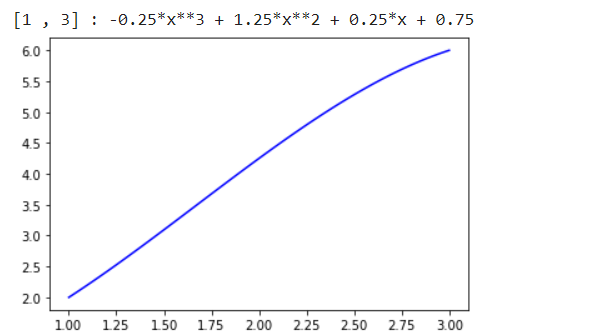
\includegraphics[width=10cm]{Images/contohLema1Hermite.png}
        \caption{Hasil interpolasi Hermite kubik $\{(1,2,2),(3,6,1)\}$ menggunakan \textit{Python}}
        \label{Gambar3.4}
    \end{figure}
    Interpolasi dicari dengan menggunakan bahasa pemrograman \textit{Python}. Dalam hal ini, diperoleh grafik hasil interpolasinya yaitu Gambar \ref{Gambar3.4}. Diperhatikan bahwa hasil grafik interpolasi Hermite kubik yang diperoleh monoton sesuai dengan Lema \ref{lema1}.
\end{contoh}

Setelah sebelumnya ditinjau syarat cukup polinomial Hermite kubik $P_i$ monoton ketika $(\alpha_i + \beta_i - 2) \leq 0$, selanjutnya akan ditinjau syarat cukup polinomial Hermite kubik $P_i$ monoton ketika $(\alpha_i + \beta_i - 2) > 0$.

\begin{lemma}\label{lema2}
    Jika  $(\alpha_i + \beta_i - 2) > 0$ dan syarat perlu monoton pada Teorema \ref{perluMonoton} terpenuhi, maka polinomial Hermite kubik $P_i(x)$ monoton pada $[x_i,x_{i+1}]$ jika dan hanya jika salah satu dari kondisi berikut terpenuhi
    \begin{enumerate}
        \item $2\alpha_i+\beta_i-3 \leq 0$,
        \item $\alpha_i+2\beta_i-3 \leq 0$,
        \item $\phi(\alpha_i, \beta_i) > 0$, dengan $ \phi(\alpha,\beta) = \alpha - \frac{1}{3}\frac{(2\alpha + \beta -3)^2}{\alpha + \beta - 2}$.
    \end{enumerate}
\end{lemma}
\begin{proof}
Ketika $(\alpha_i + \beta_i - 2) > 0$. Diperhatikan bahwa $\alpha_i$ dan $\beta_i$ selalu bernilai nonnegatif ketika syarat perlu monoton pada Teorema \ref{perluMonoton} terpenuhi. $P_i'(x)$ berdasarkan Persamaan \eqref{taylorHermite2} mempunyai titik ekstremum di
\begin{equation}\label{3.6}
    x^\star = x_i + \frac{h_i}{3}[\frac{2\alpha_i + \beta_i - 3}{\alpha_i + \beta_i - 2}],
\end{equation}
dan
\begin{equation}
    P_i'(x^\star) = \phi(\alpha_i,\beta_i)m_i,
\end{equation}
dengan
\begin{equation}\label{3.7}
    \phi(\alpha,\beta) = \alpha - \frac{1}{3}\frac{(2\alpha + \beta -3)^2}{\alpha + \beta - 2}.
\end{equation}
$P_i(x)$ monoton jika dan hanya jika salah satu dari kondisi berikut terpenuhi
\begin{enumerate}
    \item $x^\star \notin [x_i,x_{i+1}]$,
    \item $x^\star \in [x_i,x_{i+1}]$ dan $sign(P_i'(x^\star))=sign(m_i)$.
\end{enumerate}

Diperoleh dari Persamaan \eqref{3.6} kondisi pertama dapat dituliskan sebagai $x^\star > x_{i+1}$ atau $x^\star < x_{i}$ yang apabila dijabarkan diperoleh
        \begin{align*}
             &&x^\star < x_i \\
             &\Rightarrow&x_i + \frac{h_i}{3}[\frac{2\alpha_i + \beta_i - 3}{\alpha_i + \beta_i - 2}] < x_i,\\
             &\Rightarrow&\frac{h_i}{3}[\frac{2\alpha_i + \beta_i - 3}{\alpha_i + \beta_i - 2}] < 0,\\
             &\Rightarrow&2\alpha_i+\beta_i-3 < 0,
        \end{align*}
dan
\begin{align*}
             &&x^\star > x_i \\
             &\Rightarrow&x_i + \frac{h_i}{3}[\frac{2\alpha_i + \beta_i - 3}{\alpha_i + \beta_i - 2}] > x_i + h_i,\\
             &\Rightarrow&\frac{h_i}{3}[\frac{2\alpha_i + \beta_i - 3}{\alpha_i + \beta_i - 2}] > h_i,\\
             &\Rightarrow&2\alpha_i + \beta_i - 3 > 3\alpha_i+3\beta_i-6,\\
             &\Rightarrow&\alpha_i+2\beta_i-3 < 0.
        \end{align*} 
Sedangkan untuk kondisi kedua dari Persamaan \eqref{3.7} dapat diartikan bahwa $$\phi(\alpha_i, \beta_i) > 0,$$
\end{proof}
sehingga diperoleh
\begin{align*}
    &&\phi(\alpha_i, \beta_i) > 0, \\
    &\Rightarrow&\alpha_i - \frac{1}{3}\frac{(2\alpha_i + \beta_i -3)^2}{\alpha_i + \beta_i - 2}>0, \\
    &\Rightarrow&-\alpha_i(3(\alpha_i + \beta_i -2)) + (2\alpha_i + \beta_i - 3)^2 < 0, \\
    &\Rightarrow&-3\alpha_i^2 - 3 \alpha_i\beta_i + 6 \alpha_i + 4\alpha_i^2 + 4\alpha_i\beta_i - 12\alpha_i + \beta_i^2 - 6\beta_i + 9 < 0, \\
    &\Rightarrow&\alpha_i^2 + \beta_i^2 + \alpha_i\beta_i - 6\alpha_i -6\beta_i + 9 < 0, \\
    &\Rightarrow&\alpha_i^2 + \alpha_i(\beta_i - 6) + (\beta_i - 3)^2 < 0,
\end{align*}
yang merupakan daerah didalam elips dengan pusat $(2,2)$. 
\begin{figure}[H]
    \centering
    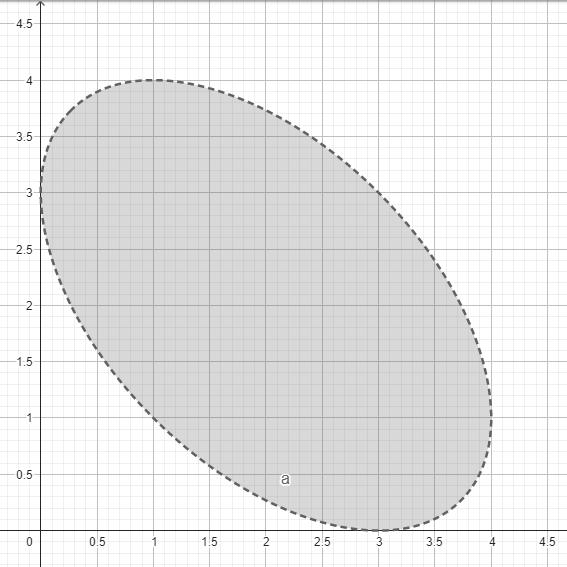
\includegraphics[width=10cm]{Images/daerahMonotonElips.png}
    \caption{Daerah elips $\alpha_i^2 + \alpha_i(\beta_i - 6) + (\beta_i - 3)^2 < 0$, dengan sumbux-$x$ adalah $\alpha$ dan sumbu-$y$ adalah $\beta$}
    \label{fig:my_label}
\end{figure}


\begin{contoh}
     Diberikan set data $\{(1,2,1),(2,4,4)\}$ sehingga $m_i=2$, $\alpha_i=0.5$ dan $\beta_i=2$. Dari situ diperoleh $\alpha_i+\beta_i-2=0.5>0$ dan $2\alpha_i+\beta_i-3 = 0 $ yang berdasarkan Lema \ref{lema2} hasil interpolasi Hermite kubiknya monoton.
     \begin{figure}[H]
         \centering
         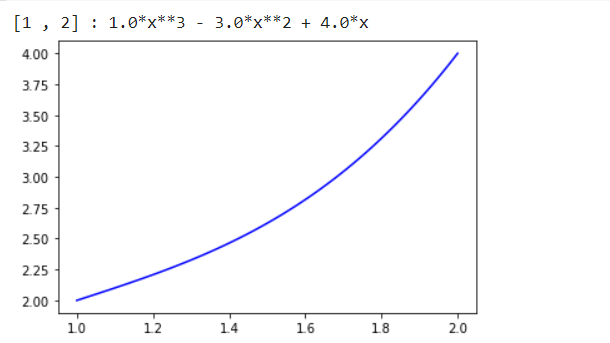
\includegraphics[width=10cm]{Images/contohLema2.1Hermite.png}
         \caption{Hasil interpolasi Hermite kubik $\{(1,2,1),(2,4,4)\}$ menggunakan \textit{Python}}
         \label{Gambar3.6}
     \end{figure}
     Untuk kondisi kedua dipilih set data $\{(1,2,4),(2,4,1)\}$ sehingga $m_i=2$, $\alpha_i=2$ dan $\beta_i=0.5$. Dari situ diperoleh $\alpha_i+\beta_i-2=0.5>0$ dan \mbox{$\alpha_i+2\beta_i-3 = 0 $} sehingga berdasarkan Lema \ref{lema2} dapat disimpulkan hasil interpolasi Hermite kubiknya monoton.
     \begin{figure}[H]
         \centering
         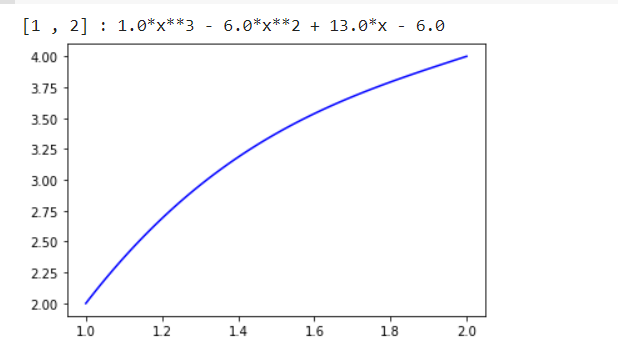
\includegraphics[width=10cm]{Images/contohLema2.2Hermite.png}
         \caption{Hasil interpolasi Hermite kubik $\{(1,2,4),(2,4,1)\}$ menggunakan \textit{Python}}
         \label{Gambar3.7}
     \end{figure}
     Terakhir, untuk kondisi ketiga dipilih set data $\{(1,2,4),(2,4,2)\}$ sehingga $m_i=2$, $\alpha_i=2$ dan $\beta_i=1$. Dari situ diperoleh $\alpha_i+\beta_i-2=1>0$ dan 
     $$\phi(\alpha_i,\beta_i) = 2 - \frac{1}{3}\frac{(2)^2}{1}=\frac{8}{3}>0,$$ sehingga interpolasi Hermite kubiknya yang dihasilkan monoton.
     \begin{figure}[H]
         \centering
         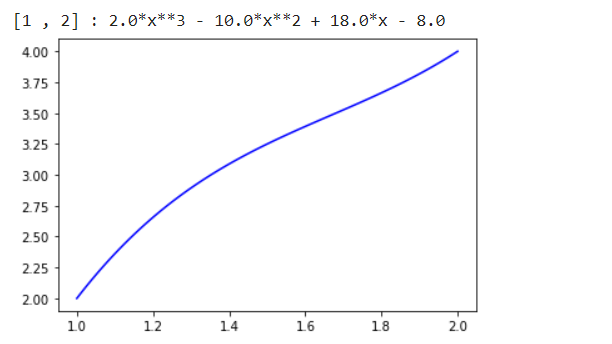
\includegraphics[width=10cm]{Images/contohLema2.3Hermite.png}
         \caption{Hasil interpolasi Hermite kubik $\{(1,2,4),(2,4,2)\}$ menggunakan \textit{Python}}
         \label{Gambar3.8}
     \end{figure}

     Pada ketiga contoh yang diberikan, diperoleh hasil interpolasi monoton pada Gambar \ref{Gambar3.6}, Gambar \ref{Gambar3.7}, dan Gambar \ref{Gambar3.8}. Hal ini sesuai dengan yang diberikan pada Lema \ref{lema2}.
\end{contoh}

Dari kedua lema yang baru saja diberikan dapat dibentuk daerah monoton berdasarkan nilai $\alpha_i$ dan $\beta_i$.

\begin{figure}[H]
    \centering
    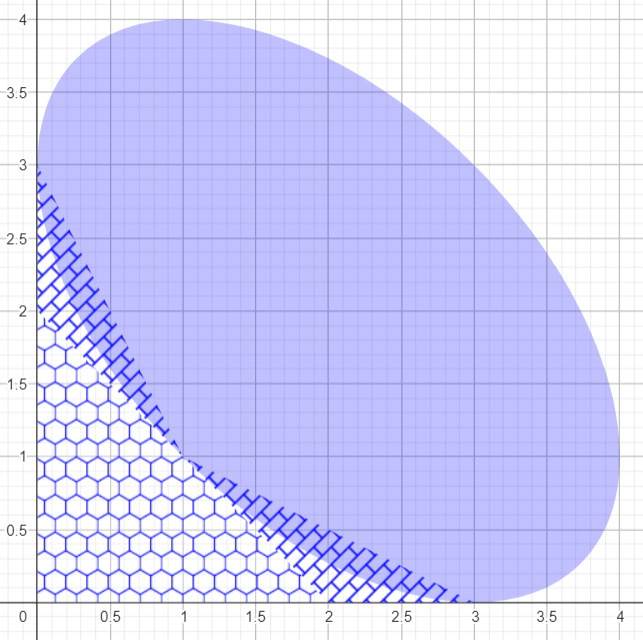
\includegraphics[width=10cm]{Images/Daerah monoton}
    \caption{Daerah Monoton Berdasarkan $\alpha_i$ dan $\beta_i$, dengan sumbux-$x$ adalah $\alpha$ dan sumbu-$y$ adalah $\beta$}
    \label{daerahmonoton}
\end{figure}

Kondisi untuk $\alpha_i$ dan $\beta_i$ yang diperoleh pada Lema \ref{lema1} dan Lema \ref{lema2} dapat digambarkan sebagai daerah arsiran pada Gambar \ref{daerahmonoton} dengan sumbu absis merupakan $\alpha_i$ dan sumbu ordinat merupakan $\beta_i$. Daerah yang diarsir merupakan daerah saat fungsi $P_i(x)$ monoton sesuai dengan Lema \ref{lema1} dan Lema \ref{lema2}.

\begin{teorema}\label{ab_leq3}
    Misal $I_i = [x_i,x_{i+1}]$ dan $P_i$ adalah polinomial hasil interpolasi Hermite kubik dari data $\{(x_i,f_i,\dot{f_i}),(x_{i+1},f_{i+1},\dot{f_{i+1}})\}$.
    Jika
    \begin{equation*}
        0 \leq \alpha_i, \beta_i \leq 3,
    \end{equation*}
    maka polinomial $P_i$ monoton pada $I_i$.
\end{teorema}

\begin{proof}
    Diperhatikan pada Gambar \ref{daerahmonoton} yang dibuat berdasarkan hasil Lema \ref{lema1} dan Lema \ref{lema2}, $0 \leq \alpha_i, \beta_i \leq 3$ berada pada daerah arsiran sehingga polinomial $P_i$ monoton pada $I_i$.
\end{proof}

\begin{teorema}\label{3.1.7}
    Misal $I_i = [x_i,x_{i+1}]$ dan $P_i$ adalah polinomial Hermite kubik yang menginterpolasi data $\{(x_i,f_i,\dot{f_i}),(x_{i+1},f_{i+1},\dot{f_{i+1}})\}$.
    Jika syarat perlu monoton
    \begin{align*}
     sign(\dot{f_i})=sign(\dot{f_{i+1}})=sign(m_i),
    \end{align*}
    untuk setiap $i=1,\dots,n-1$ terpenuhi dan
    \begin{equation*}
        |\dot{f_i}| \leq 3 \min(|m_{i-1}|,|m_i|)
    \end{equation*}
    untuk setiap $i=2,\dots,n-1$, maka polinomial $P_i$ monoton pada semua interval $I_i$, $i=1,\:2,\dots,\:n-1$.
\end{teorema}

\begin{proof}
    Diketahui untuk setiap $i=1,\:2,\dots,\:n-1$
    \begin{align*}
     sign(\dot{f_i})=sign(\dot{f_{i+1}})=sign(m_i),
    \end{align*}
    dan
    \begin{equation*}
        |\dot{f_i}| \leq 3 \min(|m_{i-1}|,|m_i|),
    \end{equation*}
    akibatnya diperoleh
    \begin{equation*}
        0 \leq \frac{\dot{f_i}}{m_i} \leq 3,
    \end{equation*}
    dan
    \begin{equation*}
        0 \leq \frac{\dot{f_{i+1}}}{m_i} \leq 3,
    \end{equation*}
    sedemikian hingga berlaku untuk setiap $i=1,\:2,\dots,\:n-2$
    \begin{equation*}
        0 \leq \alpha_i, \beta_i \leq 3.
    \end{equation*}
    Berdasarkan Teorema \ref{ab_leq3} diperoleh $P_i$ monoton pada setiap interval $I_i$ untuk setiap $i=1,\:2,\dots,\:n-2$.
\end{proof}

\begin{teorema}
    Misal $I_i = [x_i,x_{i+1}]$ dan $P_i$ adalah polinomial Hermite kubik yang menginterpolasi data $\{(x_i,f_i,\dot{f_i}),(x_{i+1},f_{i+1},\dot{f_{i+1}})\}$.
    Jika salah satu dari kondisi berikut terpenuhi
    \begin{enumerate}
        \item $0 \leq \alpha_i + \beta_i \leq 3$,
        \item $\alpha_i^2 + \alpha_i(\beta_i-6) + (\beta_i-3)^2 < 0,$
    \end{enumerate}
    $\forall i = 0, \dots, n-1$ maka polinomial $P_i$ monoton pada $I_i$.
\end{teorema}

\begin{proof}
Diperhatikan bahwa kondisi pertama merupakan daerah di dalam arsiran pada Gambar \ref{daerahmonoton} sehingga $P_i$ monoton pada $[x_i, x_{i+1}]$.
Untuk kondisi kedua berdasarkan Lema \ref{lema2} yaitu jika $\phi(\alpha_i, \beta_i) > 0$, dengan
\begin{equation}
    \phi(\alpha,\beta) = \alpha - \frac{1}{3}\frac{(2\alpha + \beta -3)^2}{\alpha + \beta - 2}
\end{equation}
maka polinomial Hermite kubik $P_i$ yang menginterpolasi data $\{(x_i,f_i,\dot{f_i}),(x_{i+1},f_{i+1},\dot{f_{i+1}})\}$ monoton pada interval $[x_i, x_{i+1}]$. Diperoleh,
\begin{align*}
    &&\phi(\alpha_i, \beta_i) > 0, \\
    &\Rightarrow&\alpha_i - \frac{1}{3}\frac{(2\alpha_i + \beta_i -3)^2}{\alpha_i + \beta_i - 2}>0, \\
    &\Rightarrow&-\alpha_i(3(\alpha_i + \beta_i -2)) + (2\alpha_i + \beta_i - 3)^2 < 0, \\
    &\Rightarrow&-3\alpha_i^2 - 3 \alpha_i\beta_i + 6 \alpha_i + 4\alpha_i^2 + 4\alpha_i\beta_i - 12\alpha_i + \beta_i^2 - 6\beta_i + 9 < 0, \\
    &\Rightarrow&\alpha_i^2 + \beta_i^2 + \alpha_i\beta_i - 6\alpha_i -6\beta_i + 9 < 0, \\
    &\Rightarrow&\alpha_i^2 + \alpha_i(\beta_i - 6) + (\beta_i - 3)^2 < 0,
\end{align*}

 Dapat disimpulkan bahwa jika kondisi kedua terpenuhi, maka $P_i$ monoton pada $[x_i, x_{i+1}]$.
\end{proof}
\begin{lemma}\label{orderAkurasi}
    Misal $f(x)$ fungsi yang mulus. Jika $\dot{f_i}=f'(x_i) + O(h^{q_i})$ dan $\dot{f_{i+1}}=f'(x_{i+1}) + O(h^{q_{i+1}})$, maka polinomial interpolasi Hermite kubik sepotong-sepotong pada interval $[x_i,x_{i+1}]$ memenuhi,
    \begin{equation*}
        P_i(x) = f(x) + O(h^q)
    \end{equation*}
    dengan $q=\min(4, q_i+1, q_{i+1}+1)$.
\end{lemma}

\begin{proof}
    Pertama-tama diambil dari Persamaan \eqref{errorHermiteKubik} diperoleh polinomial interpolasi $P_i$ memiliki order akurasi $O(h^4)$ untuk $\dot{f_i}=f'(x_i)$ dan $\dot{f_{i+1}}=f'(x_{i+1})$ sehingga
    \begin{align*}
        f(x) = P_i(x) + O(h^4).
    \end{align*}
    Diperhatikan apabila disubtitusikan $\dot{f_i}=f'(x_i) + O(h^{q_i})$ dan \mbox{$\dot{f_{i+1}}=f'(x_{i+1}) + O(h^{q_{i+1}})$} pada polinomial interpolasi Hermite kubik seperti pada Persamaan \eqref{PersHermiteKubik}, maka diperoleh
    \begin{align*}
        f(x) =& f_i + (f'(x_i) + O(h^{q_i}))(x-x_i) + \frac{(m_i-(f'(x_i) + O(h^{q_i}))}{h_i}(x-x_i)^2 \\
        &+ \frac{((f'(x_{i+1}) + O(h^{q_{i+1}}))+(f'(x_i) + O(h^{q_i}))-2m_i)}{h_i^2}(x-x_i)^2(x-x_{i+1}) + O(h^4) \\
        =& P_i(x) + O(h^{q_i})(x-x_i) + \frac{O(h^{q_i})}{h_i}(x-x_i)^2 \\
        &+ \frac{(O(h^{q_i}) + O(h^{q_{i+1}}))}{h_i^2}(x-x_i)^2(x-x_{i+1}) + O(h^{4}),
    \end{align*}
    yang berakibat
    \begin{gather*}
        f(x)\leq P_i(x) + O(h^{q_i+1}) + O(h^{q_i+1}) + O(h^{\min(q_i+1,q_{i+1}+1)}) + O(h^{4}),
    \end{gather*}
    sehingga dapat disimpulkan
    \begin{equation*}
        P_i(x) = f(x) + O(h^q),
    \end{equation*}
    dengan $q=\min(4, q_i+1, q_{i+1}+1)$.
\end{proof}

\begin{contoh}
Dipilih fungsi $f(x) = \sin(x)$ pada interval $[0,1]$. Interval tersebut dibagi menjadi beberapa subinterval. Jika $\dot{f} = f'(x)=\cos(x)$, maka akan ditinjau hasil galat dari interpolasi Hermite kubik pada titik $x=0,3$ yang memiliki order akurasi $O(h^4)$ sehingga dengan simulasi menggunakan bahasa pemrograman \textit{Python} diperoleh hasil galat dari interpolasinya.

\begin{table}[htp]
        \centering
        \begin{tabular}{|c|c|c|c|c|c|}
    \hline $h$& galat di $x = 0.3$ \\ 
    \hline
0.5&$3.84021 \times 10^{-5}$  \\
0.25&$1.46615 \times 10^{-6}$ \\
0.125&$1.78698 \times 10^{-7}$  \\
0.0625&$4.57581 \times 10^{-9}$  \\
    \hline
    \end{tabular}
        \caption{Interpolasi Hermite kubik dari fungsi $f(x)=\sin(x)$ di titik $x=0.3$, dengan turunan analitik}
        \label{contohOrderAkurasi1}
\end{table}
    
Selanjutnya, akan dibandingkan apabila nilai dari $\dot{f}$ merupakan hasil pendekatan dengan menggunakan metode beda bagi tengah yang memiliki order akurasi $O(h^2)$ sehingga hasil polinomial interpolasi yang diperoleh memiliki order akurasi $O(h^3)$ berdasarkan Lema \ref{orderAkurasi}.
\begin{table}[htp]
        \centering
        \begin{tabular}{|c|c|c|c|c|c|}
    \hline $h$& galat di $x = 0.3$ \\ 
    \hline
0.5&$0.00256163$  \\
0.25&$0.000250525 $ \\
0.125&$1.65053 \times 10^{-5}$  \\
0.0625&$3.68918 \times 10^{-6}$  \\
    \hline
    \end{tabular}
        \caption{Interpolasi Hermite kubik dari fungsi $f(x)=\sin(x)$ di titik $x=0.3$, dengan menggunakan metode beda bagi tengah}
        \label{contohOrderAkurasi2}
\end{table}
Terakhir akan ditinjau ketika nilai $\dot{f}$ dicari dengan menggunakan metode beda bagi maju yang mempunyai order akurasi $O(h)$ sehingga polinomial interpolasi yang dihasilkan memiliki order akurasi $O(h^2)$.

\begin{table}[htp]
        \centering
        \begin{tabular}{|c|c|c|c|c|c|}
    \hline $h$& galat di $x = 0.3$  \\ 
    \hline
0.5&$0.011013$  \\
0.25&$0.000758064 $ \\
0.125&$2.01257 \times 10^{-5}$  \\
0.0625&$6.50661 \times 10^{-5}$  \\
    \hline
    \end{tabular}
        \caption{Interpolasi Hermite kubik dari fungsi $f(x)=\sin(x)$ di titik $x=0.3$, dengan menggunakan metode beda bagi maju}
        \label{contohOrderAkurasi3}
\end{table}
Diperhatikan bahwa, Tabel \ref{contohOrderAkurasi1} memiliki galat yang paling kecil dibandingkan dua tabel lain yang diberikan. Tabel \ref{contohOrderAkurasi3} memiliki galat yang paling besar dibandingkan dua tabel lainnya. Hal ini sesuai dengan yang diberikan pada Lema \ref{orderAkurasi}.
\end{contoh}

